\chapter{Building calculation workflows}\label{ch:workflows}
\index{Workflows}

A workflow organizes structure preparation, electronic structure solving, and result display into a readable, reusable graph. It can handle a simple SCF run or combine symmetry analysis, band structure, density of states, and geometry optimization. This chapter introduces workflow editing, then develops common calculations for silicon and hydrogen.

If you completed Chapter~\ref{ch:first}, continue with the silicon examples. \file{examples/silicon-tutorial.ks} contains SCF and DOS workflows for an eight-atom silicon cell; \file{examples/silicon-band-primitive.ks} contains band and symmetry workflows for a two-atom primitive cell; and \file{examples/h2-tutorial.ks} contains hydrogen SCF and geometry optimization. Reference results are saved in these projects so that you can inspect them before rerunning.

\section{Edit a workflow}

\subsection{How nodes organize tasks}
\index{Workflow nodes}

Each canvas node represents a task. Select it and choose \ui{Workflow → Configure Node}, or click its gear, to expand the \ui{Config Editor} and open or refresh the task-specific \ui{Options}. Scroll down to inspect parameters. ``Configure a node'' below refers to this procedure. Modules group functions by processing stage; the task determines the actual operation. The label is simply the name shown on the canvas and can be changed for clarity.

For example, a node labeled ``Build silicon model'' can perform \ui{Build Molecule}, while ``Electronic self-consistency'' can perform \ui{SCF}. Renaming does not change the task type. Choose the correct task first, then rename it if useful.

Connections define processing order. Downstream tasks need upstream data: a band calculation needs self-consistent density and a path; a convergence plot needs an iteration history. Do not create cycles. Geometry optimization already manages repeated solves internally and does not need a canvas connection back to itself.

\subsection{Choose a starting workflow}

\ui{Import workflow from template} offers SCF, Energy Band, DOS, Relaxation, and Symmetry. Templates demonstrate common task combinations. After opening one, select the calculation structure and check parameters before running. With several structures in a project, explicitly select the intended object in the structure-input node.

Start blank for a customized workflow. Add nodes, adjust their input and output ports, connect them, and assign tasks. Zoom, fit-to-view, Undo, and Redo help organize the canvas. A clear layout makes dependencies easier to inspect.

\begin{steps}
\item Create a blank workflow and add its first node.
\item Select the node and choose \ui{Workflow → Configure Node}, then set its module and task.
\item Add the next node and connect it in processing order.
\item Configure structures, physical parameters, and numerical settings in turn.
\item Name and save the workflow, then validate it with a small calculation.
\end{steps}

\subsection{Projects and workflow files}

A \file{.ks} project retains structures, workflows, results, and other contents. A \file{.wf} file stores one graph and its task settings for reuse across projects. When sharing a \file{.wf}, also supply the structure and explain how to select it as input.

Save the project for complete day-to-day work. Export a workflow when you want to reuse a calculation method on another system, then adjust the structure and accuracy settings for that system.

\section{Choose a task}\label{sec:task-catalog}

Templates provide common combinations; the task list provides the operations available to individual nodes. \ui{Module} first chooses the processing stage, then \ui{Task} selects its function. Each node performs one task, chosen in the Config Editor.

\begin{longtable}{p{.28\linewidth}p{.65\linewidth}}
\caption{Workflow tasks and their roles.}\label{tab:task-catalog}\\
\toprule
Module and task & Purpose and required inputs \\
\midrule
\endfirsthead
\toprule
Module and task & Purpose and required inputs (continued) \\
\midrule
\endhead
Preprocessing & \ui{Symmetry \& K-Path}: analyze crystal symmetry and generate a high-symmetry path from the selected structure. \\
Computation & \ui{Build Molecule}: convert a project structure into a calculation object and set functional, pseudopotentials, cutoff, and sampling. \\
Computation & \ui{SCF}: find a self-consistent density and produce ground-state energy, electronic states, and iteration history. \\
Computation & \ui{NSCF}: prepare options for later band or DOS calculations. This node alone does not produce a new band plot. \\
Computation & \ui{Geometry Optimization}: update atomic positions through electronic calculations; requires a complete ground-state specification. \\
Computation & \ui{TDDFT}: prepare a Casida excited-state calculation from ground-state electronic states. See the excited-state section for parameters and solving. \\
Postprocessing & \ui{Band Calculation}: generate $k$ points along a symmetry path and solve non-self-consistently; needs SCF results, NSCF options, and a symmetry path. \\
Postprocessing & \ui{Band Calculation 3D}: sample a reciprocal-space plane; needs SCF results and NSCF options. \\
Visualization & \ui{Energy Curve}: plot SCF energy and error histories. \\
Visualization & \ui{Band Structure}: plot the path bands produced by Band Calculation. \\
Visualization & \ui{Band Structure 3D}: plot energy surfaces from Band Calculation 3D. \\
Visualization & \ui{DOS}: use an NSCF grid to calculate and display total density of states. \\
Visualization & \ui{Brillouin Zone 2D}: display a 2D Brillouin zone and path from symmetry results. \\
Visualization & \ui{Brillouin Zone 3D}: display a 3D Brillouin zone and path from symmetry results. \\
\bottomrule
\end{longtable}

Task names match the interface. Preprocessing defines geometry and paths, computation prepares electronic structure, postprocessing samples the resulting states, and visualization presents data. DOS also performs grid sampling within its own task, so a module name alone does not tell you whether numerical calculation is required.

\section{Add node ports}

Top ports accept preceding connections; bottom ports connect to subsequent nodes. A 0-0 node has no ports, a 0-1 node has only a bottom port, a 1-0 node has only a top port, and a 1-1 node has both. These are canvas connection patterns, not different solvers.

\begin{steps}
\item Activate a blank workflow and add a 0-1 node from \ui{Workflow → Add Node}.
\item Configure \ui{Computation Module → Build Molecule} and select an imported structure.
\item Add two 1-1 nodes for \ui{SCF} and \ui{Energy Curve}; the latter is in \ui{Visualization Module}.
\item Drag from each preceding node's bottom port to the next node's top port to connect the three.
\item If a node has the wrong port pattern, select it and add or remove top/bottom ports through Edit Node. Check connections before removing a port in use.
\item Use Zoom In, Zoom Out, and Fit to View to inspect the complete graph, then save.
\end{steps}

Check each node's task and parameters before running SCF. Undo and Redo restore graph edits. Save a \file{.wf} to import the same graph into another project later.

\section{Understand general node settings}

\ui{General} contains the label, module, and task. \ui{Options} and \ui{Advanced Options} contain task parameters. Changing tasks replaces the parameter set; it does not convert the previous task's values into new ones. Select the task before entering its settings.

The editor also shows \ui{Inputs}, \ui{Resources}, and \ui{Outputs}. Resource execution mode, process count, and thread count affect actual execution. Input-access and output-save/forward checkboxes do not filter results, and the resource time-limit field does not stop a task automatically. View results under \ui{Results} and save the project to retain them.

\section{Allocate node resources}\label{sec:node-resources}
\index{Parallel computing}

\subsection{Node order and parallel work within a node}

Nodes run in the dependency order defined by connections. Drawing two branches does not make those branches execute simultaneously. Parallelism within a node divides parts of a task among computing processes, such as distributing NSCF $k$ points. These are different execution concepts.

Select a node, choose \ui{Workflow → Configure Node}, and expand \ui{Resources} to see its supported execution modes. Choices depend on the task and the diagonalization method selected by \ui{DiagMethod}.

\begin{table}[!htb]
\centering
\caption{Node resource fields.}
\label{tab:node-resource-fields}
\begin{tabularx}{\linewidth}{lX}
\toprule
Field & Meaning \\
\midrule
Parallel environment & Choose \ui{Serial}, \ui{Parallel (process pool)}, \ui{GPU (diagonalization)}, or \ui{Use NSCF settings} for a supported follow-up task. Available choices depend on the task.\\
Maximum processes & Positive integer, default 2. Limits pool workers; editable only in process-pool mode.\\
Threads/process & Positive integer, default 1. Limits CPU computational threads per process; editable in pool or GPU mode.\\
Time limit & No Limit, 30 minutes, 1 hour, or 2 hours. This field does not trigger automatic stopping.\\
\bottomrule
\end{tabularx}
\end{table}

A worker is a calculation process. A maximum of 2 processes with 1 thread/process allows at most two workers, each with at most one CPU computational thread. The main application still runs its interface and schedules tasks, so these values do not count every operating-system process or thread. More workers also need more memory and may not speed up a small exercise.

\ui{Serial} disables the node's pool and GPU calculation paths; it does not force all CPU work onto one core. Numerical libraries may still use their own threads. Threads/process does not select a thread-based parallel pool: node pools use process workers.

\subsection{Check task support}

\begin{table}[!htb]
\centering
\caption{Resource choices for common tasks.}
\label{tab:node-resource-support}
\begin{tabularx}{\linewidth}{p{.29\linewidth}X}
\toprule
Task & Available execution modes \\
\midrule
SCF & Serial; GPU for supported diagonalizers. No process-pool option.\\
NSCF & Serial; process pool with HT interpolation disabled, and GPU for supported methods. Later band and DOS tasks can inherit these settings.\\
Band Calculation, DOS & Serial, inherited NSCF settings, process pool, and supported GPU methods. Pool and GPU modes are unavailable with HT interpolation.\\
Band Calculation 3D & Serial, inherited NSCF settings, process pool, and supported GPU methods. Direct NSCF sampling is used, without HT interpolation.\\
Other tasks & Currently serial, including structure construction, symmetry, geometry optimization, TDDFT, and general plotting.\\
\bottomrule
\end{tabularx}
\end{table}

GPU options support \texttt{lobpcg}, \texttt{davidson}, \texttt{davidson2}, and \texttt{davpcg}. The default SCF \texttt{davidson\_qe} is not among them, so a newly opened SCF resource panel may offer only Serial. GPU acceleration applies to supported diagonalization steps; other work retains its own execution mode. Threads/process in GPU mode limits CPU-side computational threads. The device manages GPU kernel threads.

Band and DOS tasks use the preceding NSCF diagonalization options, so check its \ui{DiagMethod} and \ui{Use HT} too. A task or method change can reset an incompatible resource choice to Serial; recheck Resources before running. \ui{Use NSCF settings} displays inherited process and thread counts in noneditable fields. Change them in NSCF, or choose an independent mode in the later node.

If a workflow contains several NSCF nodes, later sampling uses the most recently executed NSCF configuration. It does not choose by canvas proximity or retain a separate configuration for each branch. Keep separate workflows when comparing resources or solver conditions so that inheritance is unambiguous.

\subsection{Exercise: two workers for silicon \headinglatin{DOS}}

Use this chapter's silicon DOS workflow without changing its structure, cutoff, grid, energy range, or step. Complete a serial reference first, then compare the execution mode so that environmental and physical changes remain distinguishable.

\begin{steps}
\item Open the silicon DOS workflow, select \ui{NSCF}, and choose \ui{Configure Node}.
\item Under \ui{Options}, keep \ui{DiagMethod} at \texttt{lobpcg} and \ui{Use HT} cleared.
\item Expand \ui{Resources}, choose \ui{Parallel (process pool)}, and enter 2 maximum processes and 1 thread/process.
\item Select \ui{DOS}, choose \ui{Use NSCF settings} in its Resources, and check the displayed counts of 2 and 1.
\item Save. Run the complete workflow in an environment with the required parallel support, inspect $k$-point messages, and check the new DOS result.
\item Record resources and timing. To compare serial execution again, set NSCF to \ui{Serial} and check that DOS still inherits it.
\end{steps}

NSCF mainly prepares solver options; it does not complete band or DOS sampling itself. The subsequent non-self-consistent sampling task actually uses the pool. A supported $k$-point loop is distributed only when there is more than one $k$ point; a single-point calculation cannot provide the same parallel benefit. \ui{Serial} disables the node's pool path while retaining an existing pool.

Resource choices do not change the physical model. Still compare convergence, sampling, and energy references; execution modes may differ in their last numerical digits. Distinguish pool startup time from solving time as well.

\begin{figure}[!htb]
\centering
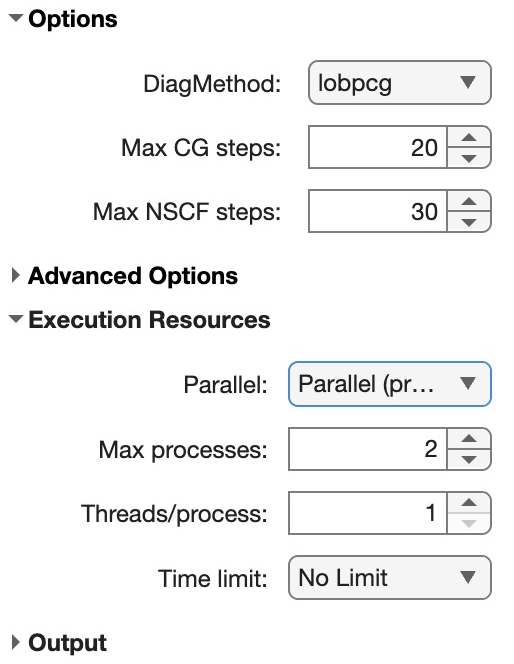
\includegraphics[width=66mm]{publication-assets/revision-nscf-process-resources.png}
\caption{NSCF process-pool settings: at most two workers, with one CPU computational thread per worker.}
\label{fig:nscf-resources-live}
\end{figure}

\begin{figure}[!htb]
\centering
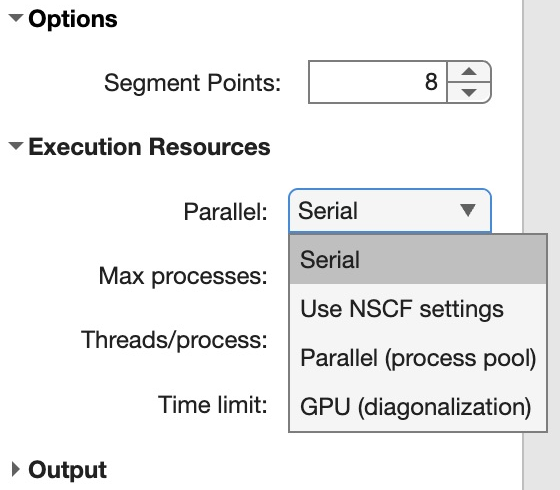
\includegraphics[width=70mm]{publication-assets/revision-band-resource-options.png}
\caption{Band Calculation can inherit NSCF settings or use its own execution mode.}
\label{fig:band-inherit-live}
\end{figure}

\FloatBarrier
\subsection{Respond to unavailable resources}

A dropdown choice indicates task support, but the execution machine must also support it. Pools need Parallel Computing Toolbox and a process-based pool configuration. GPU execution needs a supported available GPU and its calculation components. An Online browser displays the interface on your computer, but the server provides calculation resources. A disabled Home \ui{Parallel} button does not make all node parallel options unavailable; check the node and actual server environment.

If no pool exists, the application attempts to create a local process pool up to the node's maximum process count. A request above the local profile's worker limit produces an error rather than silently enlarging that limit. An existing pool is checked for type, worker count, and CPU threads per worker. Thread-based pools, oversized pools, and excessive thread counts cause conflicts. A smaller compatible pool can be reused: the maximum does not guarantee that a new pool of exactly that size is created for every task.

Begin with Serial if parallel execution is not configured, then check the environment separately. Full MATLAB\regmark{} users can close an incompatible pool they created before rerunning with node settings. The application preserves user-created pool configurations. A temporary pool created by the current node is released when that task finishes or exits.

\subsection{Use node settings remotely}

Node resources determine how a task uses computing resources; remote settings in Chapter~\ref{ch:remote} determine where the workflow is submitted. They can be used together, but entering two workers neither submits a cluster job nor changes node order.

Remote submissions carry node resource settings. A job already executing on a remote worker cannot create a nested pool automatically inside a node. Request a suitable pool at submission and ensure remote thread settings are compatible. For a node allowing at most 2 workers with 1 thread each, an existing 4-worker remote pool exceeds the limit. Check cluster worker counts, PoolSize, and node limits together.

Online CPU and memory status monitors the current session; it is not a resource-request control. Save node settings with the project. For remote work, also retain the cluster and submission conditions to reproduce the same environment later.

\section{Silicon: your first periodic calculation}

\subsection{Prepare the eight-atom silicon cell}

Silicon is a useful introduction to periodic calculations and semiconductor bands. This tutorial uses an eight-atom cubic cell with lattice constant $5.4437023729$ Å, stored in \file{examples/silicon.cif}. Similarly named files elsewhere in the software may use different lattice constants. Use the supplied file for numerical comparisons.

For a new project, follow these steps. If \file{silicon-tutorial.ks} is open, select its silicon SCF workflow and continue with the settings below.

\begin{steps}
\item Save and close existing work to return to an empty project.
\item Import \file{silicon.cif} and check eight independent silicon sites and a cubic cell.
\item Save as \file{silicon-learning.ks}.
\item Show cell boundaries as needed and rotate the model to inspect the arrangement.
\item Open the SCF template and select this silicon structure as input.
\end{steps}

A periodic viewer may show bonds across cell boundaries and neighboring images. Repeated spheres do not necessarily mean duplicate atoms were imported. Use structure information for atom counts and cell boundaries for periodic connectivity.

\subsection{Set \headinglatin{SCF} conditions}

Choose \ui{Crystal}. Unlike hydrogen, this calculation uses periodic sampling and extra empty states. A $2\times2\times2$ grid builds the density, and four additional bands provide low-energy unoccupied states. The band tutorial uses a separate standardized two-atom primitive cell; DOS retains this eight-atom cell.

\begin{table}[htbp]
\centering
\caption{Silicon tutorial SCF settings.}
\begin{tabularx}{\linewidth}{lX}
\toprule
Location & Setting\\
\midrule
Build Molecule / Type & Crystal\\
Structure & Only the supplied silicon structure\\
Functional / Pseudopotential & PBE / default\\
Ecut (Hartree) & 20\\
Smearing / Temperature & fermi-dirac / 0 K\\
Nspin & 1\\
\mbox{\ui{Autokpts}} & \mbox{\texttt{[2 2 2 0 0 0]}}\\
Extra bands & 4\\
SCF / DiagMethod & davidson\_qe\\
SCF / Max SCF steps & 100\\
\bottomrule
\end{tabularx}
\end{table}

These modest settings keep a complete periodic exercise manageable. Test cutoff and $k$-point convergence as described in Chapter~\ref{ch:theory} when greater energy, gap, or DOS accuracy is needed.

\subsection{Run and check}

Activate and run silicon SCF. Match the structure name and loaded silicon pseudopotential to the example, wait for self-consistency, then inspect the energy curve. The reference converges in seven iterations, with total energy approximately $-31.1058309605$ Ha and final relative density error approximately $7.35\times10^{-9}$.

This total energy belongs to the eight-atom cell. Normalize consistently before comparing primitive cells, supercells, or per-atom energies. The total energies of eight- and two-atom cells cannot be compared directly to decide which is lower.

\section{Silicon: bands along a high-symmetry path}
\index{Band structures}

\subsection{What the band workflow does}

A band plot shows electronic energies as functions of wavevector along representative high-symmetry directions. This is easier to interpret than a list of eigenvalues at every $k$ point. The full workflow builds the structure, analyzes symmetry, converges the density, prepares NSCF options, samples a path, and plots the result.

Use \file{examples/silicon_primitive.cif}, or open \file{examples/silicon-band-primitive.ks}. This standardized two-atom cell has three equal lattice vectors approximately $3.84928$ Å long at mutual angles of $60^\circ$. It represents the same periodic crystal as the eight-atom conventional cell. Recommended path coordinates are expressed in the standardized primitive reciprocal basis, so using that cell keeps path and calculation coordinates consistent. Start with \ui{Energy Band}. \ui{Build Molecule} supplies the structure, \ui{Symmetry \& K-Path} the path, \ui{SCF} the density, \ui{NSCF} solver options, \ui{Band Calculation} the path sampling, and \ui{Band Structure} the plot.

Symmetry and SCF may occupy different branches. Check that both kinds of information are available before band calculation rather than forcing every node into one column. Preserve template dependencies when rearranging the canvas.

\subsection{Configure symmetry and the path}
\index{Symmetry}

Select only \file{silicon_primitive} in \ui{Build Molecule}. Keep Crystal, PBE, default, 20 Ha, Nspin = 1, 0 K, the \mbox{\texttt{[2 2 2 0 0 0]}} SCF grid, and 4 extra bands. The same integer grid gives different sampling densities in primitive and conventional cells, so it does not establish equal per-atom energy accuracy. In \ui{Symmetry \& K-Path}, keep lattice threshold $10^{-7}$, symmetry precision $10^{-5}$, and angle tolerance $-1$. The reported space group should agree with the actual geometry.

The recommended path depends on the current crystal. Cell choices, small distortions, and tolerances can change it. Accept the recommendation initially and check the point labels in the result. In later strain or defect studies, path changes may themselves reflect changed symmetry.

\subsection{Choose NSCF solver options}

NSCF's \ui{DiagMethod} chooses the electronic-state solver. \ui{Max CG steps} and \ui{Max NSCF steps} limit two iteration levels, not path $k$ points. Path resolution belongs to the later Band Calculation node.

\begin{table}[htbp]
\centering
\caption{Basic NSCF options.}
\begin{tabularx}{\linewidth}{lX}
\toprule
Field & Default and meaning \\
\midrule
DiagMethod & lobpcg; follow another example's parameter table if it specifies a different method. \\
Max CG steps & 20, the internal LOBPCG iteration limit. \\
Max NSCF steps & 30, the outer NSCF iteration limit. \\
Use GACE & Cleared by default; a specialized exchange-processing option. \\
Use HT & Cleared by default; relevant to Hamiltonian transformation interpolation. \\
\bottomrule
\end{tabularx}
\end{table}

HT interpolation needs complete inputs, including ground-state wavefunctions and eigenvalues. The PBE path-band and DOS examples keep GACE and HT off and use direct NSCF sampling. Retain those inputs for advanced calculations in full MATLAB\regmark{}.

\subsection{Set NSCF and path sampling}

\begin{steps}
\item Keep SCF at davidson\_qe and at most 100 iterations.
\item Retain NSCF defaults: lobpcg, Max CG steps 20, and Max NSCF steps 30.
\item Leave \ui{Use GACE} and \ui{Use HT} cleared.
\item Set \mbox{\ui{Segment Points}} in \ui{Band Calculation} to \texttt{8}.
\item Check the final \ui{Band Structure} node and save.
\end{steps}

Eight points per segment, including both endpoints, give a quick overview. Use $20$ or more for a smoother curve. More path points mainly increase follow-up solving work; they do not replace SCF-grid convergence testing.

\subsection{Run and read the plot}

Activate and run this workflow. After SCF, the program samples the path. Wait for the plotting node to finish.

The horizontal axis lists high-symmetry points in path order. The vertical axis is energy relative to the run's Fermi energy in eV. Several occupied bands and some low-energy unoccupied bands should appear. The number of curves is the number of calculated bands, not the atom count.

\screenshot{publication-assets/vector-1d3af63f1336e902c5cd.pdf}{Reference bands for the two-atom silicon primitive cell, with 8 points per segment and the Fermi energy set to zero. Combined labels mark disconnected path segments.}{fig:si-band-results}

The reference has six recommended path segments and eight bands. Its primitive-cell SCF converges in seven iterations, at approximately $-7.6905500238$ Ha and $8.19\times10^{-10}$ final relative density error. The coarse SCF grid and short path make the workflow easy to learn. A band-gap study requires further sampling tests and identification of the band extrema.

\subsection{Make a controlled comparison}

Save the workflow as \file{.wf}, then use \ui{Import workflow from file...} to create a copy. Change only \mbox{\ui{Segment Points}} from $8$ to $20$. Check whether curves become smoother while energies at symmetry points agree. This distinguishes finer path plotting from a denser density-building grid.

Next, hold path resolution fixed and increase only \mbox{\ui{Autokpts}} in Build Molecule for SCF. That comparison tests density and potential against integration accuracy. Record both settings with each plot to explain any differences.

\section{Silicon: calculate total density of states}
\index{Density of states (DOS)}

\subsection{Why \headinglatin{DOS} needs another grid}

Bands show how electronic states vary along selected directions. DOS describes how many states are available near an energy and needs sampling throughout the Brillouin zone. It cannot be obtained by simply counting states along the high-symmetry path.

Open the \ui{DOS} template and inspect Build Molecule, SCF, NSCF, and DOS. Return to the eight-atom \file{silicon.cif} and the initial periodic SCF settings in this chapter. Primitive-cell bands and conventional-cell DOS share functional and pseudopotentials but differ in cell and sampling. Match models, sampling, and energy references for quantitative comparison. The \ui{DOS} node performs NSCF sampling on its grid and obtains total DOS by tetrahedron integration.

\subsection{Set the grid and energy range}

\begin{steps}
\item Set Build Molecule to Crystal and select this silicon structure. Keep PBE, default, 20 Ha, Nspin = 1, and 4 extra bands.
\item In \ui{Build Molecule}, set the SCF \mbox{\ui{Autokpts}} to:
\par\nobreak\noindent\mbox{\texttt{[2 2 2 0 0 0]}}.
\item Keep the NSCF solver defaults described above.
\item Set \ui{NSCF Grid} in DOS to \texttt{[4 4 4]}.
\item Set \ui{Start Energy} to \texttt{-10} eV, \ui{End Energy} to \texttt{10} eV, and \ui{Energy Step Size} to \texttt{0.05} eV.
\item Save and run the active DOS workflow.
\end{steps}

The energy step determines where DOS is evaluated along the energy axis. Reducing it refines that axis but cannot compensate for too few $k$ points. Vary these two approximations separately.

Tetrahedron DOS requires more than one grid point in each direction; this tutorial uses $4\times4\times4$. Layered and wire-like models must also meet this requirement, with convergence checked for the specific system.

\subsection{Read and check the result}

The plot places DOS horizontally and energy vertically, allowing a shared energy direction with a neighboring band plot. Other sources often place energy horizontally. Both layouts are valid; read axis labels first.

The specified range gives 401 energy samples, and DOS values are nonnegative. Peaks and fine structure change with the grid. Use a denser grid to check the stability of the principal peak positions and widths.

Figure~\ref{fig:si-dos-results} shows this example's DOS.

\subsection{Improve the \headinglatin{DOS}}

After the first run, change NSCF Grid to \texttt{[6 6 6]} or \texttt{[8 8 8]} without changing other conditions. More points substantially increase NSCF work and may stabilize peak shapes. Save the existing result before running so that the curves can be compared.

For higher unoccupied energies, increase Extra bands before expanding the energy limit. Changing End Energy from $10$ to $20$ eV does not create uncomputed states. The energy range, band count, and $k$ sampling must together cover the region of interest.

\section{Hydrogen: find a lower-energy geometry}
\index{Geometry optimization}
\index{Structural relaxation}

\subsection{Optimization versus a single-point calculation}

Chapter~\ref{ch:first} holds hydrogen positions fixed. Here, allow atoms to move to lower the total energy. Bond length is the clearest geometric measure for a diatomic molecule. Start from the same $10$ Bohr cube and $1.5$ Bohr bond, retaining PBE, default pseudopotentials, and $20$ Ha.

Open the hydrogen project and choose \ui{Relaxation}. Optimization resolves the electronic problem after every position update and costs more than one SCF run. The task manages its own geometry iterations.

\subsection{Configure optimization}

\begin{steps}
\item Select the original hydrogen structure in Build Molecule and choose Molecule.
\item Check PBE, default, 20 Ha, Nspin = 1, and 0 K against the original SCF.
\item Select \ui{Geometry Optimization}.
\item Set \ui{RelaxMethod} to \ui{fminunc}.
\item Explicitly enter \texttt{1e-4} for \ui{RelaxTolerance} and \texttt{100} for \ui{MaxRelaxSteps}.
\item Save, activate this workflow, and run it.
\end{steps}

Other methods include nlcg2, bfgs, and fire, which update positions differently. This tutorial uses fminunc. In the MATLAB\regmark{} toolbox edition, it requires Optimization Toolbox. The standalone application includes the corresponding runtime components.

\subsection{Follow the two iteration levels}

Repeated SCF sequences in the optimization log solve electronic structures at successive geometries. One converged SCF means that geometry's electronic calculation is complete, not that optimization has finished. Locate the final geometry-optimization status and check its last electronic solve.

\begin{figure}[!htb]
\centering
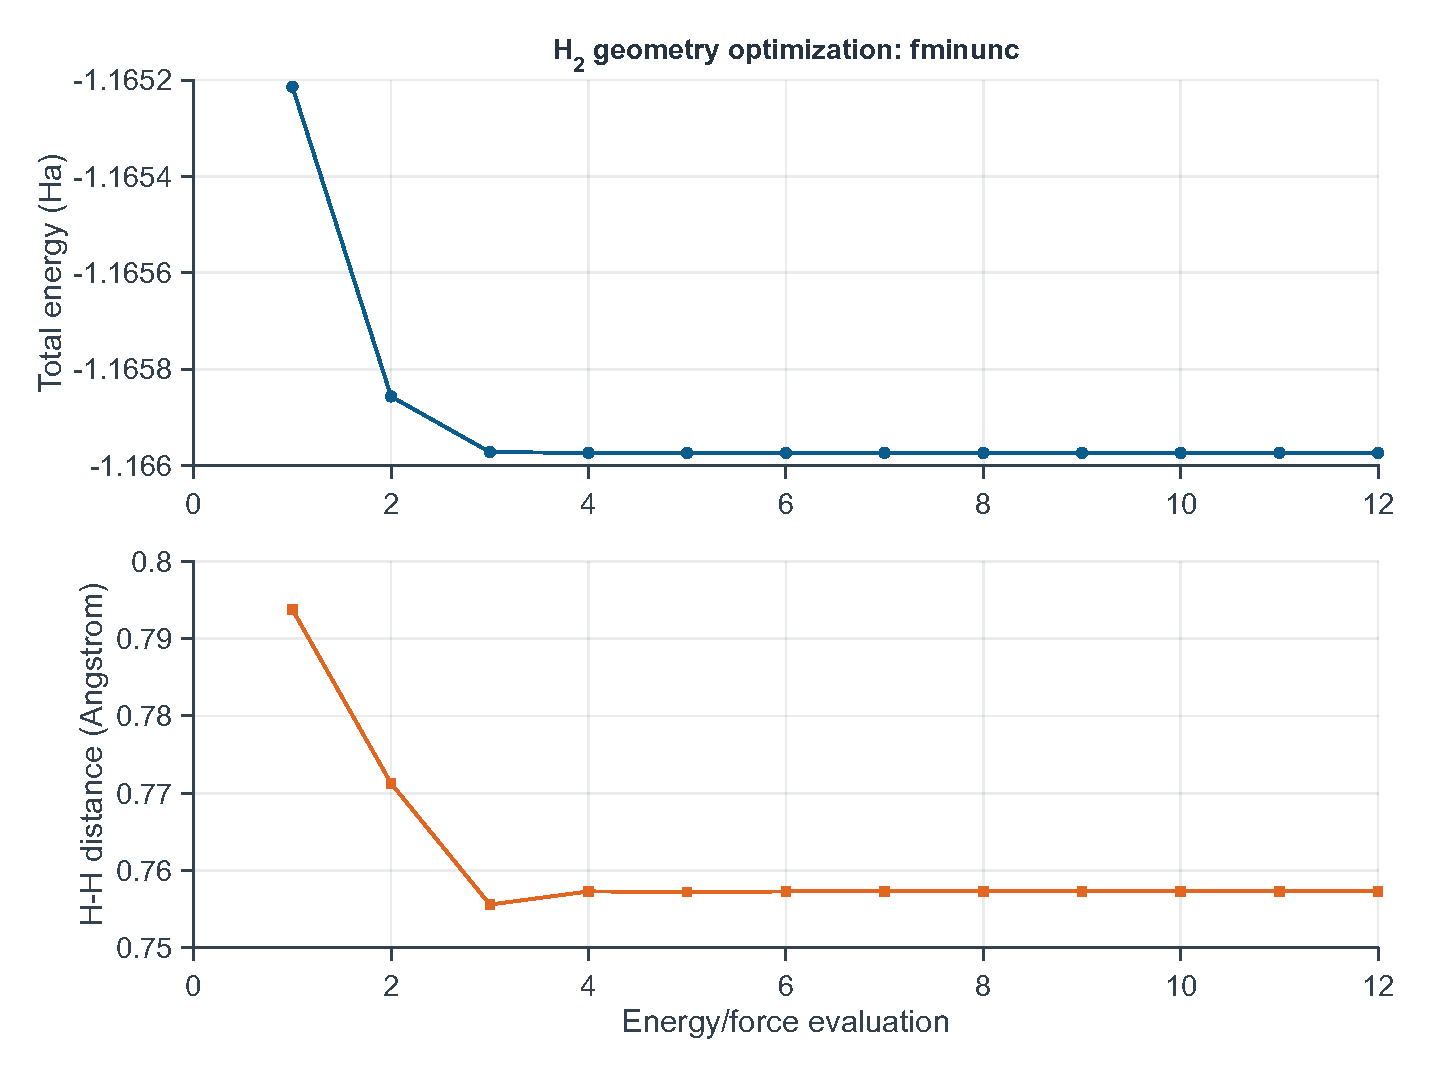
\includegraphics[width=\linewidth]{publication-assets/vector-a7002e532f8546105cf1.pdf}
\caption{Hydrogen energy and bond length during optimization. The horizontal axis counts energy/force function evaluations, including trial geometries.}
\label{fig:h2-relax-results}
\end{figure}

Function evaluations, electronic iterations, and geometry steps need not have the same count. Some methods test several positions to choose a step length. Do not count every logged energy as an accepted atomic move.

\subsection{Reference result}

With these settings, fminunc gives a final bond length of approximately $1.43107436$ Bohr, or $0.75729194$ Å. Total energy is approximately $-1.1659737582$ Ha, and the force norm approximately $5.55\times10^{-5}$ atomic units. Both optimization and the final SCF report convergence.

The bond is slightly shorter and the energy lower than initially. This result belongs to the specified box, functional, pseudopotentials, and cutoff; changing them can change the value.

Optimization records are stored with workflow results. The original model under \ui{Structure} remains unchanged. Import \file{examples/h2_optimized.cif} to measure the final bond in the 3D viewer. The accompanying script also saves an optimized structure for further analysis.

\section{Symmetry as an independent workflow}

To inspect symmetry or a recommended path alone, open \ui{Symmetry} in the two-atom primitive-cell example without performing a complete electronic calculation. This is useful after importing a crystal, building a supercell, or applying deformation.

Symmetry tolerances determine which small numerical differences in positions or lattice parameters are treated as equivalent. An overly strict tolerance can interpret rounding as reduced symmetry; an overly loose one can hide a real distortion. Begin with defaults for ideal tutorial silicon. Interpret experimental or optimized structures in light of coordinate precision.

Symmetry describes geometric relationships. Energetic stability requires electronic calculations and force checks. Read symmetry alongside optimization records when assessing a relaxed structure.

\section{View the Brillouin zone}\label{sec:bz-workflow}
\index{Brillouin zone}

A Brillouin-zone plot places the one-dimensional band path in reciprocal space. A band plot's horizontal axis gives distance along the path but not its course through the reciprocal-space polyhedron. A 3D zone plot shows boundaries, symmetry points, and paths together. This exercise needs no SCF calculation.

% Native English captures; see docs/provenance/english-edition-assets.json for source and crop metadata.
\begin{figure}[H]
\centering
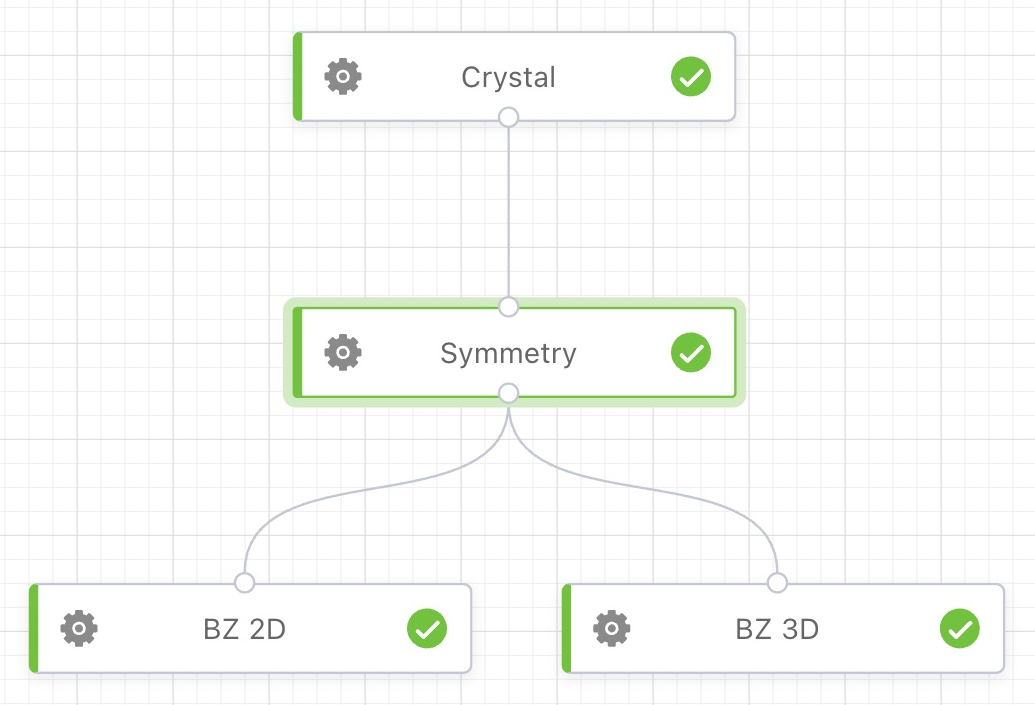
\includegraphics[width=99mm]{publication-assets/crop-7a61cf8df5b1fcc967e4.png}
\caption{The four-node \ui{Symmetry} template. \ui{Crystal} supplies the structure to \ui{Symmetry}, which passes its analysis to \ui{BZ 2D} and \ui{BZ 3D}. All four nodes show green completion markers after a successful run.}
\label{fig:si-symmetry-online}
\end{figure}


\begin{steps}
\item Import \file{silicon_primitive.cif} and confirm a two-site primitive cell under \ui{Structure}. Choose \ui{Home → Workflow → Import workflow from template → Symmetry}.
\item Keep the template's four nodes: \ui{Crystal} supplies the structure, \ui{Symmetry} analyzes it, and branches lead to \ui{BZ 2D} and \ui{BZ 3D}. Check the inputs before changing anything.
\item Open \ui{Crystal} with its gear. Confirm \ui{Build Molecule}, type \ui{Crystal}, and only \file{silicon_primitive} under \ui{Choose imported structures}. Keep PBE, default pseudopotentials, 20 Ha, 0 K, and Nspin=1. These create a crystal object; this workflow has no SCF task.
\item Open \ui{Symmetry} and confirm \ui{Symmetry \& K-Path}, \ui{SymmetryThreshold} \texttt{1e-7}, and \ui{SymmetryPrecision} \texttt{1e-5}; retain other defaults. Open \ui{BZ 3D} and confirm \ui{Visualization Module → Brillouin Zone 3D}. It has no further task-specific parameters.
\item Keep this workflow active and choose \ui{Home → Run}. Both plotting branches produce results. Neither a preceding SCF nor deletion of \ui{BZ 2D} is needed.
\item Explicitly open \ui{BrillouinZone3D} under \ui{Results → Plots}. Use this entry if the 2D plot appears first.
\item Rotate the plot to identify zone boundaries, reciprocal axes, and $\Gamma$, X, U, W, K, and L. Follow paths between front and rear faces, and compare the labels and segments with the same primitive-cell band tutorial.
\item Save the project and, in Online, download the \file{.ks}. To use the plot in a report, choose the toolbar's image export action, save the image separately, and retain the project.
\end{steps}

% Original Online result export: preserve vector paths and embedded fonts.
\begin{figure}[H]
\centering
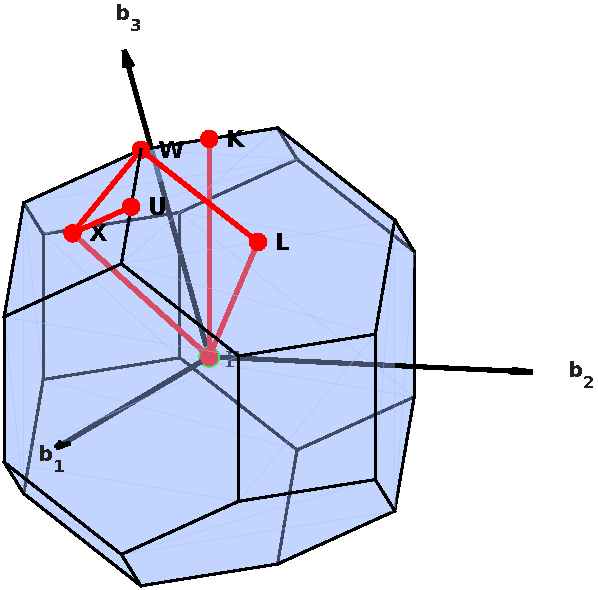
\includegraphics[width=95mm]{publication-assets/vector-cc7185e6fa1fba4c8c34.pdf}
\caption{The two-site silicon primitive cell's 3D Brillouin zone. The \ui{Symmetry} template produces a blue boundary polyhedron, a red high-symmetry path, and black reciprocal-axis arrows. Rotate to inspect $\Gamma$, X, U, W, K, L, and their connections. No SCF calculation is required.}
\label{fig:si-bz-online}
\end{figure}


Figure~\ref{fig:si-bz-online} shows the 3D zone. The supplied \file{Si-primitive-BZ-Online-050.pdf} is a vector figure retaining path lines, point labels, and reciprocal axes for enlargement and reports.

\ui{BZ 2D} uses \ui{Brillouin Zone 2D}, plotting plane information from the first two reciprocal vectors. Use it in a separate workflow for a 2D model with well-defined in-plane vectors. It does not convert an arbitrary oblique section of a 3D crystal into a 2D material. Focus on the 3D view for silicon here, and use a suitably oriented 2D lattice for later 2D exercises. Cell, path, and symmetry choices for both plotting tasks are configured upstream.

Reopen the saved project and check the figure, structure, and path before using its views in a report.

\section{Plot band-energy surfaces}\label{sec:band-surface}
\index{Band-energy surfaces}

Path bands sample line segments; an energy surface samples a reciprocal-space plane and uses height for electronic energy. This helps reveal directional variation near a band edge. Here, ``3D'' means two sampling coordinates and one energy coordinate, not a full 3D $k$-point volume. It also differs from the real-space volumetric data in Chapter~\ref{ch:volume}.

Prepare a separate project using \file{silicon_primitive.cif}. Keep Crystal, PBE, default, 20 Ha, and the primitive-cell SCF grid; set 4 extra bands to include unoccupied states. A small-range exercise uses a non-spin-polarized insulator so that the highest occupied and lowest unoccupied bands are clear.

\begin{steps}
\item Save a copy of the SCF project and retain \ui{Build Molecule → SCF}.
\item Append \ui{NSCF}, \ui{Band Calculation 3D}, and \ui{Band Structure 3D}. The middle task is Postprocessing and the last Visualization.
\item Keep the tutorial NSCF options. Enter the center, plane, and grid below in Band Calculation 3D.
\item Save and run. The workflow first solves the ground state, then samples the plane non-self-consistently, so it can take longer than SCF alone.
\item If calculation completes, open \ui{EnergyBandStructure3D} under Results. Rotate the two band-edge surfaces, inspect their relationship to the sampling plane, and save.
\end{steps}

\begin{table}[htbp]
\centering
\caption{A small-grid band-surface example.}
\begin{tabularx}{\linewidth}{lX}
\toprule
Option & Input and meaning \\
\midrule
Center KPoint & \literalinput{[0 0 0]}, centered near Gamma. \\
Slice Plane & XY; alternatives are XZ and YZ. \\
Slice Plane Grid & \literalinput{[5 5]}, five points per direction, 25 in total. \\
Plane Grid Spacing & 0.015, controlling this task's sampling extent. This is a reciprocal-space parameter, not an interatomic distance. \\
\bottomrule
\end{tabularx}
\end{table}

The five points in each direction span 0.0375 on either side of the center, including both endpoints. Plane Grid Spacing controls the extent in this task. Record the center, plane, point counts, and extent when comparing surfaces quantitatively.

The plotting task selects the highest occupied and lowest unoccupied bands and sets the run's Fermi energy to zero. These surfaces show band-edge dispersion. Axis ticks may be absent, so use sampling data for quantitative analysis and test grid and range convergence.

\section{Prepare an excited-state calculation}\label{sec:tddft-workflow}
\index{TDDFT}

SCF gives ground-state electronic structure. Excitations in response to a small perturbation require a different calculation. The TDDFT task prepares Casida-method inputs from converged ground-state states with enough unoccupied orbitals. Replacing the last SCF task with TDDFT while retaining occupied orbitals only does not provide the required excitation space.

\subsection{Retain unoccupied hydrogen orbitals}

Start from Chapter~\ref{ch:first}'s \file{h2.cif} in a separate project, with Molecule, PBE, default, 20 Ha, and Nspin=1. Set \ui{Extra bands} to 4 in Build Molecule's advanced options, then run SCF. The neutral hydrogen molecule has one doubly occupied spatial orbital, and four extra bands provide the later unoccupied-orbital selection. They do not change atom count or charge.

Add a Computation \ui{TDDFT} node after SCF. Select it, choose \ui{Configure Node}, and inspect Options and Advanced Options.

\begin{table}[htbp]
\centering
\caption{Preparatory hydrogen TDDFT settings.}
\begin{tabularx}{\linewidth}{lX}
\toprule
Field & Choice and meaning \\
\midrule
TDDFTMethod & casida, the method provided by this task. \\
DiagMethod & direct, direct diagonalization. \\
nvbands & 1 occupied orbital. \\
ncbands & 4 unoccupied orbitals; cannot exceed those obtained in the ground-state calculation. \\
nroots & 3 requested excited states; no greater than $nvbands\times ncbands$. \\
Use TDA & Selected for the Tamm--Dancoff approximation. \\
Use IPA / Use RPA & Both cleared here; use separately to compare response approximations. \\
\bottomrule
\end{tabularx}
\end{table}

Explicitly enter \ui{nvbands}=1 and \ui{ncbands}=4. The solver requires Nspin=1. Check ground-state extra bands together with any changes in occupied bands, unoccupied bands, or root count. To retain a degenerate group of transitions, the program may increase the final number of roots. Use the actual count in logs and output arrays for analysis.

\begin{notebox}{How to solve TDDFT}
A parameter-passing issue in the graphical TDDFT node prevents it from completing this excited-state solve. Prepare the ground state and excitation space above, then pass explicit name/value arguments in full MATLAB\regmark{} as below to obtain excitation energies and transition vectors. The associated message is \texttt{Wrong input for tddft\_input}.
\end{notebox}

\subsection{Pass explicit parameters in full \headinglatin{MATLAB}\regmark{}}

The following code assumes an initialized KSSOLV numerical environment in full MATLAB\regmark{}. It reruns the ground state with four extra bands, then passes Casida arguments explicitly. Inspect ground-state convergence, excitation energies, and transition vectors afterward.

\noindent\begin{minipage}{\linewidth}
\begin{lstlisting}[language=Matlab]
pseudopotential.PpType('default');
molecule = example.structure.H2();
molecule.ecut = 20;
molecule.funct = 'PBE';
molecule.extranbnd = 4;
scfOptions = options.SCF();
scfOptions.enableGPU = false;
scfOptions.enableParallelPool = false;
[molecule, H, X, scfInfo] = scf(molecule, scfOptions);
if ~scfInfo.converge
    error('Ground-state SCF did not converge.');
end
td = tddft_setup(molecule, scfOptions, H, X, ...
    'method', 'casida', 'diag', 'direct', ...
    'nvbands', 1, 'ncbands', 4, 'nroots', 3, ...
    'istda', true, 'isipa', false, 'isrpa', false);
[excitationHa, transitionVectors] = ...
    tddft_casida_direct(td, molecule);
save('h2-tddft.mat', 'excitationHa', ...
    'transitionVectors', 'scfInfo', 'td');
\end{lstlisting}
\end{minipage}

Excitation energies are returned in Ha; use the manual's conversion for eV. Transition vectors describe orbital combinations in an excitation. They are not directly an absorption spectrum with intensities and broadening. Interpret excitations with the ground-state conditions, selected bands, response approximation, and original outputs.

\section{Make workflows reproducible and comparable}

\subsection{Give each workflow a clear purpose}

While learning, keep separate ``Silicon SCF,'' ``Silicon bands,'' and ``Silicon DOS'' workflows. Each then has an obvious purpose and run target. Combine or export personal templates once you are comfortable.

After copying a workflow by saving and reimporting \file{.wf}, check its structure selection. Saved settings may retain associations with the original structure. Change Build Molecule first for a new system, then inspect its model parameters. A renamed workflow still calculates its selected input.

\subsection{Document one change at a time}

Short names such as ``Silicon DOS, 4×4×4'' and ``Silicon DOS, 8×8×8'' distinguish comparisons. Record the SCF grid, extra bands, energy range, and step in result notes. This keeps figures recognizable without losing reproducibility.

An old plot does not become a result for new settings when a node is edited. Rerun and check which new datasets and figures belong to the latest calculation. Retain useful comparisons and remove redundant or abandoned trials so that the project remains readable.

\subsection{Final workflow checks}

Reopen the saved project and check the structure, node parameters, and results in turn. Confirm that the calculation object and method match the description and that results can still be read. For bands and DOS, retain the path or grid and the energy reference too.
